\documentclass[tikz,border=5pt]{standalone}
\usepackage{luatexja}
\usepackage[hiragino-pron]{luatexja-preset}
\usepackage{amsmath,amssymb}
\usepackage{pgfplots}
\pgfplotsset{compat=1.18}
\usetikzlibrary{arrows.meta,calc,decorations.markings,patterns,positioning}

% Common styles
\tikzset{
  axis/.style={-{Stealth[length=6pt]}, thick},
  curve/.style={thick, red},
  dashed curve/.style={thick, dashed, blue},
  dot/.style={circle, fill, inner sep=1.5pt},
  open dot/.style={circle, draw, fill=white, inner sep=1.5pt},
}

\begin{document}
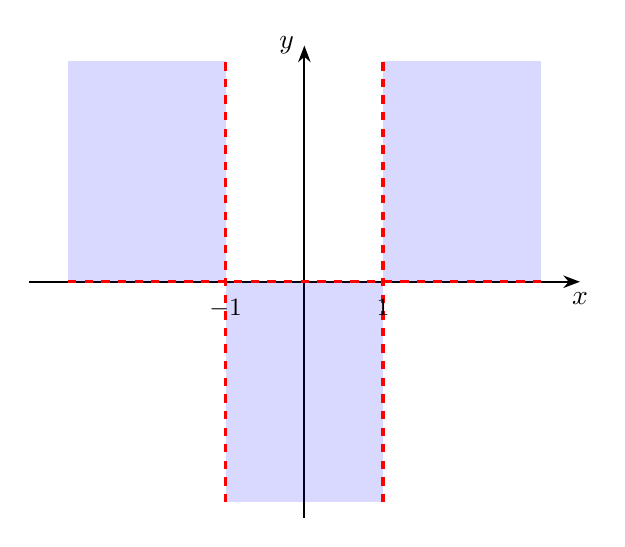
\begin{tikzpicture}
  % Axes
  \draw[axis] (-3.5,0) -- (3.5,0) node[below] {$x$};
  \draw[axis] (0,-3) -- (0,3) node[left] {$y$};

  % Region where y/(x^2-1) > 0
  % Case 1: x^2 > 1 and y > 0 (x < -1 or x > 1, y > 0)
  \fill[blue, opacity=0.15] (-3,0) rectangle (-1,2.8);
  \fill[blue, opacity=0.15] (1,0) rectangle (3,2.8);

  % Case 2: x^2 < 1 and y < 0 (-1 < x < 1, y < 0)
  \fill[blue, opacity=0.15] (-1,0) rectangle (1,-2.8);

  % Boundary lines x = ±1 (excluded)
  \draw[red, dashed, very thick] (-1,-2.8) -- (-1,2.8);
  \draw[red, dashed, very thick] (1,-2.8) -- (1,2.8);

  % y = 0 line (excluded)
  \draw[red, dashed, very thick] (-3,0) -- (3,0);

  % Labels
  \node[below, font=\small] at (-1,-0.1) {$-1$};
  \node[below, font=\small] at (1,-0.1) {$1$};
\end{tikzpicture}
\end{document}
